\documentclass[conference]{IEEEtran}

% ------------------------------------------------
% Packages
% ------------------------------------------------
\usepackage{cite}
\usepackage{amsmath,amssymb,amsfonts}
\usepackage{graphicx}
\usepackage{textcomp}
\usepackage{xcolor}
\usepackage{url}
\usepackage{tabularx}
\usepackage{array}
\usepackage{booktabs}
\usepackage{ragged2e}
\usepackage{algorithm}
\usepackage{algpseudocode}
\usepackage{tikz}
\usetikzlibrary{positioning,arrows.meta,shapes.geometric,calc}
\usepackage{hyperref} % keep hyperref last

% ------------------------------------------------
% Table configuration
% ------------------------------------------------
\newcolumntype{L}[1]{>{\RaggedRight\arraybackslash}p{#1}}
\newcolumntype{Y}{>{\RaggedRight\arraybackslash}X}

% ------------------------------------------------
% TikZ styles used by the architecture figures
% ------------------------------------------------
\tikzset{
    comp/.style={draw, rounded corners=2pt, fill=white, align=center,
        font=\scriptsize, minimum height=0.75cm, inner sep=2pt,
        text width=#1},
    comp/.default=2.7cm,
    layer/.style={draw, rounded corners=4pt, line width=0.6pt},
    ltitle/.style={font=\scriptsize\bfseries, anchor=north west,
        inner sep=3pt},
    arr/.style={-{Stealth[length=2mm]}, line width=0.6pt},
    darr/.style={{Stealth[length=2mm]}-{Stealth[length=2mm]},
        line width=0.6pt},
    lbl/.style={font=\tiny, fill=white, inner sep=1pt},
    fcstep/.style={draw, rounded corners=2pt, align=center,
        fill=blue!5, font=\scriptsize, minimum height=0.7cm,
        inner sep=2pt, text width=#1},
    fcstep/.default=4.0cm,
    fcdec/.style={draw, diamond, aspect=2.4, align=center,
        fill=orange!12, font=\scriptsize, inner sep=1pt},
    fcside/.style={draw, rounded corners=2pt, align=center,
        fill=gray!12, font=\scriptsize, inner sep=2pt,
        text width=2.4cm}
}

% ------------------------------------------------
% Document
% ------------------------------------------------
\begin{document}

\title{AI-Powered College Information Chatbot for Engineering Aspirants in Karnataka Using Hybrid RAG Architecture}

\author{
    \IEEEauthorblockN{Ajay Kumar S}
    \IEEEauthorblockA{\textit{USN: 1MS24IS400} \\
    \textit{Dept. of Information Science and Engineering} \\
    \textit{M. S. Ramaiah Institute of Technology}\\
    Bengaluru, Karnataka, India }
    \and
    \IEEEauthorblockN{Karthik S Poojary}
    \IEEEauthorblockA{\textit{USN: 1MS23IS051} \\
    \textit{Dept. of Information Science and Engineering} \\
    \textit{M. S. Ramaiah Institute of Technology}\\
    Bengaluru, Karnataka, India}
}

\maketitle

% ------------------------------------------------
% Abstract
% ------------------------------------------------
\begin{abstract}
Selecting an appropriate engineering college is an important
decision for students participating in the Karnataka Common
Entrance Test (KCET) admission process. Aspirants must examine
lengthy official cutoff documents published by the Karnataka
Examinations Authority (KEA), which list closing ranks for every
college, course, and reservation category. Extracting relevant
information from these documents manually is time-consuming and
may lead to misinterpretation of numerical or institution-specific
details.

This paper presents an AI-powered college information chatbot
based on a Hybrid Retrieval-Augmented Generation (RAG)
architecture. The official KCET 2026 Round-1 provisional cutoff
document (69 pages) is parsed into 56,610 structured
college--course--category records covering 242 colleges and
37 reservation categories. Each record with a published closing
rank is converted into a self-contained text document. Dense
retrieval is implemented using 768-dimensional Gemini embeddings
stored in PostgreSQL with the pgvector extension, while sparse
retrieval uses BM25 with domain-specific acronym expansion. The
two rankings are combined using Reciprocal Rank Fusion (RRF).
Rank-based eligibility questions are additionally answered through
deterministic SQL filtering over the structured records, so that
numerical comparisons are not delegated to the language model.
The retrieved evidence is supplied to Google Gemini to generate
context-grounded responses with page-level source references.

The system is designed to help engineering aspirants understand
published cutoff information. It provides information-based
decision support rather than attempting to predict or guarantee
future admission outcomes.
\end{abstract}

\begin{IEEEkeywords}
Retrieval-Augmented Generation, Hybrid Retrieval,
BM25, Dense Retrieval, Reciprocal Rank Fusion,
College Information System, KCET, pgvector,
Educational Chatbot.
\end{IEEEkeywords}

% ------------------------------------------------
% 1. INTRODUCTION
% ------------------------------------------------
\section{Introduction}

The selection of an engineering college is a significant
decision for students completing their pre-university
education. In Karnataka, students participating in the
Karnataka Common Entrance Test (KCET) admission process
must evaluate multiple institutions, engineering branches,
reservation categories, and cutoff ranks before
making informed choices.

The information required for this decision is published
by KEA as large PDF documents. A single cutoff document
contains thousands of rows in which each row corresponds
to a college and course, and each column corresponds to one
of 37 reservation categories. Students frequently need to
search through these documents and interpret numerical
records manually, which is tedious and error-prone.

Large Language Models (LLMs) provide a natural-language
interface for answering user questions. However, relying
only on their internal knowledge can produce inaccurate
or outdated responses. Retrieval-Augmented Generation
(RAG), introduced by Lewis et al. \cite{Lewis2020},
addresses this limitation by retrieving relevant external
information and providing it as context to a language
generation model.

Traditional information retrieval methods also have
limitations. Sparse retrieval methods such as BM25
\cite{Robertson2009} are effective for exact keyword
matching, college codes, branch names, and category
codes. However, they may not retrieve semantically
related documents when users phrase their questions
differently.

Dense retrieval methods represent queries and documents
using embedding vectors. They can identify semantically
related content even when the exact words differ.
The Dense Passage Retrieval approach proposed by
Karpukhin et al. \cite{Karpukhin2020} demonstrates
the effectiveness of dense representations for
open-domain question answering.

To address the limitations of individual retrieval
methods, this work proposes a hybrid RAG architecture
that combines dense and sparse retrieval. The retrieved
results are merged using Reciprocal Rank Fusion
\cite{Cormack2009}, allowing the system to benefit
from both semantic similarity and exact keyword matching.
Numerical admission queries are additionally handled through
structured database filtering to avoid relying on generated
text for exact numerical comparisons.

The major contributions of this work are:

\begin{itemize}
    \item Development of a domain-specific college
    information chatbot for engineering aspirants
    in Karnataka, built over the official KEA cutoff
    document.

    \item An ingestion pipeline that converts the
    multi-column cutoff tables into structured records
    and record-level text documents with page metadata.

    \item Integration of dense semantic retrieval
    and sparse BM25 retrieval, combined through
    Reciprocal Rank Fusion.

    \item Use of deterministic SQL filtering for
    rank-based and category-specific eligibility
    queries.

    \item Generation of evidence-grounded responses
    whose source references are derived from record
    metadata rather than from model output.
\end{itemize}

% ------------------------------------------------
% 2. LITERATURE SURVEY
% ------------------------------------------------
\section{Literature Survey}

Research related to the proposed system can be divided
into four major areas: retrieval-augmented generation,
information retrieval techniques, hybrid retrieval
methods, and educational chatbot applications.

\subsection{Retrieval-Augmented Generation}

Lewis et al. \cite{Lewis2020} introduced Retrieval-Augmented
Generation, combining a pre-trained language generation
model with an external non-parametric memory. Their work
demonstrated that retrieved information can improve
performance on knowledge-intensive natural language
processing tasks.

Guu et al. \cite{REALM2020} proposed Retrieval-Augmented
Language Model Pre-Training (REALM), which integrates
a knowledge retriever into the language model
pre-training process. Their work established the
importance of retrieving external knowledge instead
of relying entirely on information stored in model
parameters.

Izacard and Grave \cite{FiD2021} proposed Fusion-in-Decoder
(FiD), a retrieval-based question-answering approach
that processes multiple retrieved passages and combines
their information during generation. Their findings
highlight the importance of using multiple evidence
passages for knowledge-intensive question answering.

Borgeaud et al. \cite{RETRO2022} introduced the
Retrieval-Enhanced Transformer (RETRO), which retrieves
relevant document chunks from a large external corpus
during language generation. Their work demonstrated
that retrieval can improve language modelling without
requiring an excessively large parametric model.

\subsection{Sparse and Dense Information Retrieval}

Robertson and Zaragoza \cite{Robertson2009} presented
the Probabilistic Relevance Framework and discussed
BM25, one of the most widely used sparse information
retrieval algorithms. BM25 ranks documents according
to term frequency, inverse document frequency, and
document-length normalization. This makes it useful
for queries containing exact terms, identifiers, and
technical expressions.

Karpukhin et al. \cite{Karpukhin2020} introduced
Dense Passage Retrieval (DPR), which uses a
dual-encoder architecture to represent questions
and passages in a shared vector space. Their work
demonstrated that dense retrieval can outperform
traditional sparse retrieval on several open-domain
question-answering benchmarks.

Khattab and Zaharia \cite{ColBERT2020} proposed
ColBERT, a retrieval architecture based on contextualized
late interaction. It independently encodes queries
and documents and performs fine-grained token-level
similarity matching during retrieval.

Thakur et al. \cite{BEIR2021} introduced the BEIR
benchmark for evaluating information retrieval models
across heterogeneous datasets. Their study found that
BM25 remains a strong baseline, while reranking and
late-interaction approaches can provide improved
retrieval effectiveness at higher computational costs.

Gao et al. \cite{HyDE2023} proposed Hypothetical
Document Embeddings (HyDE), a zero-shot dense retrieval
approach that generates a hypothetical document from
a query and uses its embedding to identify relevant
documents. This work explores ways to improve semantic
retrieval without requiring query-document relevance
labels.

\subsection{Hybrid Retrieval and Retrieval Optimization}

Cormack et al. \cite{Cormack2009} introduced Reciprocal
Rank Fusion (RRF), a method for combining rankings
produced by multiple information retrieval systems.
RRF uses the reciprocal of the rank position to
calculate a combined score, making it possible to
merge rankings without requiring their original
scores to be calibrated.

Sawarkar et al. \cite{BlendedRAG2024} proposed
Blended RAG, combining dense vector retrieval,
sparse retrieval, and hybrid query strategies.
Their work demonstrates the potential of combining
multiple retrieval signals for generative
question-answering systems.

Jiang et al. \cite{FLARE2023} introduced Forward-Looking
Active Retrieval Augmented Generation (FLARE), which
performs iterative retrieval during generation when
the model requires additional information. Their
approach highlights the role of retrieval decisions
in improving long-form generation.

Asai et al. \cite{SelfRAG2024} proposed Self-RAG,
which uses retrieval and self-reflection to improve
the factuality and relevance of generated responses.
The approach evaluates whether retrieval is required
and whether retrieved evidence supports the generated
answer.

Yan et al. \cite{CRAG2024} proposed Corrective
Retrieval-Augmented Generation (CRAG), which evaluates
the quality of retrieved documents and initiates
corrective retrieval actions when the evidence is
insufficient or unreliable.

\subsection{Evaluation and Educational Applications}

Es et al. \cite{RAGAS2023} introduced RAGAS, a
reference-free evaluation framework for RAG systems.
It evaluates different components of a RAG pipeline,
including retrieval relevance, faithfulness, and
answer quality.

Saad-Falcon et al. \cite{ARES2024} proposed ARES,
an automated evaluation framework that measures
context relevance, answer faithfulness, and answer
relevance. Their work provides a systematic approach
for evaluating retrieval-augmented generation systems.

Yang et al. \cite{CRAGBenchmark2024} introduced the
Comprehensive RAG Benchmark (also abbreviated CRAG,
distinct from Corrective RAG \cite{CRAG2024}), which
contains question-answer pairs across multiple domains
and question categories. The benchmark highlights that
even advanced RAG systems can struggle with
dynamic, less popular, and complex factual questions.

Liu et al. \cite{LostMiddle2024} investigated how
language models use information within long input
contexts. Their findings show that model performance
can decrease when relevant information is positioned
in the middle of lengthy contexts. This motivates
careful retrieval and context selection rather than
simply supplying large amounts of text.

Swacha and Gracel \cite{EducationSurvey2025} surveyed
RAG chatbot applications in education. Their study
examined educational use cases, knowledge domains,
underlying language models, and evaluation methods.
The survey demonstrates the growing application of
RAG-based systems in educational environments.

Li et al. \cite{EducationalRAG2025} presented a
systematic survey of RAG applications in education.
Their work discusses retrieval, indexing, generation,
interactive learning systems, educational content
generation, and the challenges of hallucination,
knowledge completeness, and computational cost.

Lang and Gürpinar \cite{LearningSupport2025}
investigated the effectiveness of a RAG chatbot
in an online programming course. Their study
examined student interactions and satisfaction,
demonstrating the potential of course-specific
RAG systems to support educational activities.

\subsection{Research Gap}

The reviewed studies establish the effectiveness
of RAG, dense retrieval, sparse retrieval, and
hybrid ranking for knowledge-intensive question
answering. Educational surveys also demonstrate
the growing relevance of domain-specific RAG
chatbots.

However, the problem of helping engineering
aspirants interpret institution-specific and
numerical admission information requires additional
considerations. College codes, branch identifiers,
reservation categories, and cutoff ranks require
precise matching and structured filtering.

A purely semantic retrieval system may retrieve
conceptually relevant information without guaranteeing
exact numerical matching. Conversely, keyword-based
retrieval may fail when users express their questions
using different terminology. Furthermore, the source
data is tabular, so conventional fixed-length text
chunking would separate a closing rank from the college,
course, and category to which it belongs.

The proposed system addresses these requirements
by using record-level documents, combining dense
semantic retrieval with BM25-based keyword retrieval
and rank fusion, and answering rank-eligibility
questions with structured SQL queries.

% ------------------------------------------------
% 3. COMPARISON TABLE
% ------------------------------------------------
\section{Comparison of Related Works}

Table~\ref{tab:literature_comparison} summarizes
21 research works related to retrieval-augmented
generation, information retrieval, hybrid retrieval,
RAG evaluation, and educational applications.

The comparison identifies the primary contribution
of each work and its relevance to the proposed
college information chatbot.

\begin{table*}[!t]
\centering
\caption{Comparison of Related Research Works}
\label{tab:literature_comparison}

\scriptsize
\renewcommand{\arraystretch}{1.16}
\setlength{\tabcolsep}{3pt}

\begin{tabularx}{\textwidth}{
    L{2.25cm}
    L{2.55cm}
    L{3.15cm}
    Y
}
\toprule
\textbf{Reference} &
\textbf{Research Area} &
\textbf{Method / Technique} &
\textbf{Contribution and Relevance} \\
\midrule

Lewis et al. (2020) \cite{Lewis2020} &
Knowledge-intensive QA &
Retrieval-Augmented Generation &
Introduced RAG by combining parametric language models with an external knowledge index. Establishes the foundation of the proposed system. \\

Guu et al. (2020) \cite{REALM2020} &
Knowledge retrieval &
REALM &
Integrated a latent knowledge retriever into language model pre-training, demonstrating the importance of external knowledge retrieval. \\

Robertson and Zaragoza (2009) \cite{Robertson2009} &
Information retrieval &
BM25 and probabilistic relevance framework &
Explained BM25 ranking and its probabilistic foundations. Supports the sparse retrieval component. \\

Cormack et al. (2009) \cite{Cormack2009} &
Rank aggregation &
Reciprocal Rank Fusion &
Introduced RRF for combining independent search rankings without requiring score normalization. Directly relevant to hybrid retrieval. \\

Karpukhin et al. (2020) \cite{Karpukhin2020} &
Open-domain QA &
Dense Passage Retrieval &
Introduced dual-encoder dense retrieval for semantic passage matching. Supports the dense retrieval component. \\

Khattab and Zaharia (2020) \cite{ColBERT2020} &
Neural information retrieval &
ColBERT late interaction &
Proposed contextualized token-level interaction for efficient passage retrieval and fine-grained relevance matching. \\

Izacard and Grave (2021) \cite{FiD2021} &
Open-domain QA &
Fusion-in-Decoder &
Combined information from multiple retrieved passages during generation, demonstrating the value of multi-passage evidence. \\

Thakur et al. (2021) \cite{BEIR2021} &
Retrieval benchmarking &
BM25, dense retrieval, reranking &
Introduced a heterogeneous retrieval benchmark and demonstrated the importance of evaluating retrieval methods across different domains. \\

Borgeaud et al. (2022) \cite{RETRO2022} &
Language modelling &
Retrieval-Enhanced Transformer &
Used retrieved document chunks during generation to improve knowledge-intensive language modelling. \\

Gao et al. (2023) \cite{HyDE2023} &
Zero-shot retrieval &
Hypothetical Document Embeddings &
Generated hypothetical documents to improve dense retrieval without requiring relevance labels. \\

Jiang et al. (2023) \cite{FLARE2023} &
Adaptive RAG &
Forward-Looking Active Retrieval &
Introduced iterative retrieval during generation when additional evidence is required. \\

Es et al. (2024) \cite{RAGAS2023} &
RAG evaluation &
RAGAS metrics &
Proposed reference-free evaluation of retrieval relevance, faithfulness, and generated answer quality. \\

Liu et al. (2024) \cite{LostMiddle2024} &
Long-context QA &
Context-position evaluation &
Demonstrated that language models may fail to use relevant information positioned in the middle of long contexts. \\

Asai et al. (2024) \cite{SelfRAG2024} &
RAG reliability &
Self-RAG and self-reflection &
Introduced retrieval and reflection mechanisms to improve the relevance and factuality of generated responses. \\

Yan et al. (2024) \cite{CRAG2024} &
RAG reliability &
Corrective RAG &
Evaluated retrieved evidence and introduced corrective retrieval actions when the retrieved information is insufficient. \\

Saad-Falcon et al. (2024) \cite{ARES2024} &
RAG evaluation &
ARES evaluation framework &
Evaluated context relevance, answer faithfulness, and answer relevance using automated language-model judges. \\

Yang et al. (2024) \cite{CRAGBenchmark2024} &
RAG benchmarking &
Comprehensive RAG Benchmark &
Introduced a multi-domain benchmark and highlighted the difficulty of answering complex and dynamic factual questions. \\

Sawarkar et al. (2024) \cite{BlendedRAG2024} &
Hybrid retrieval &
Dense and sparse retrieval &
Proposed Blended RAG, combining semantic and keyword-based retrieval strategies for generative QA. \\

Swacha and Gracel (2025) \cite{EducationSurvey2025} &
Educational chatbots &
Survey of educational RAG systems &
Reviewed RAG chatbot applications in education, including institutional information and subject-specific knowledge systems. \\

Li et al. (2025) \cite{EducationalRAG2025} &
Educational applications &
Systematic RAG survey &
Analyzed RAG indexing, retrieval, generation, and educational applications, identifying challenges such as hallucination and outdated knowledge. \\

Lang and Gürpinar (2025) \cite{LearningSupport2025} &
Educational support &
Course-specific RAG chatbot &
Studied a RAG chatbot in an online programming course and examined student engagement and satisfaction. \\

\bottomrule
\end{tabularx}
\end{table*}

% ------------------------------------------------
% 4. SYSTEM ARCHITECTURE
% ------------------------------------------------
\section{System Architecture}

Fig.~\ref{fig:architecture} shows the overall architecture
of the proposed system. It is organised into five layers
and one offline pipeline.

\begin{figure*}[!t]
\centering
\resizebox{\textwidth}{!}{%
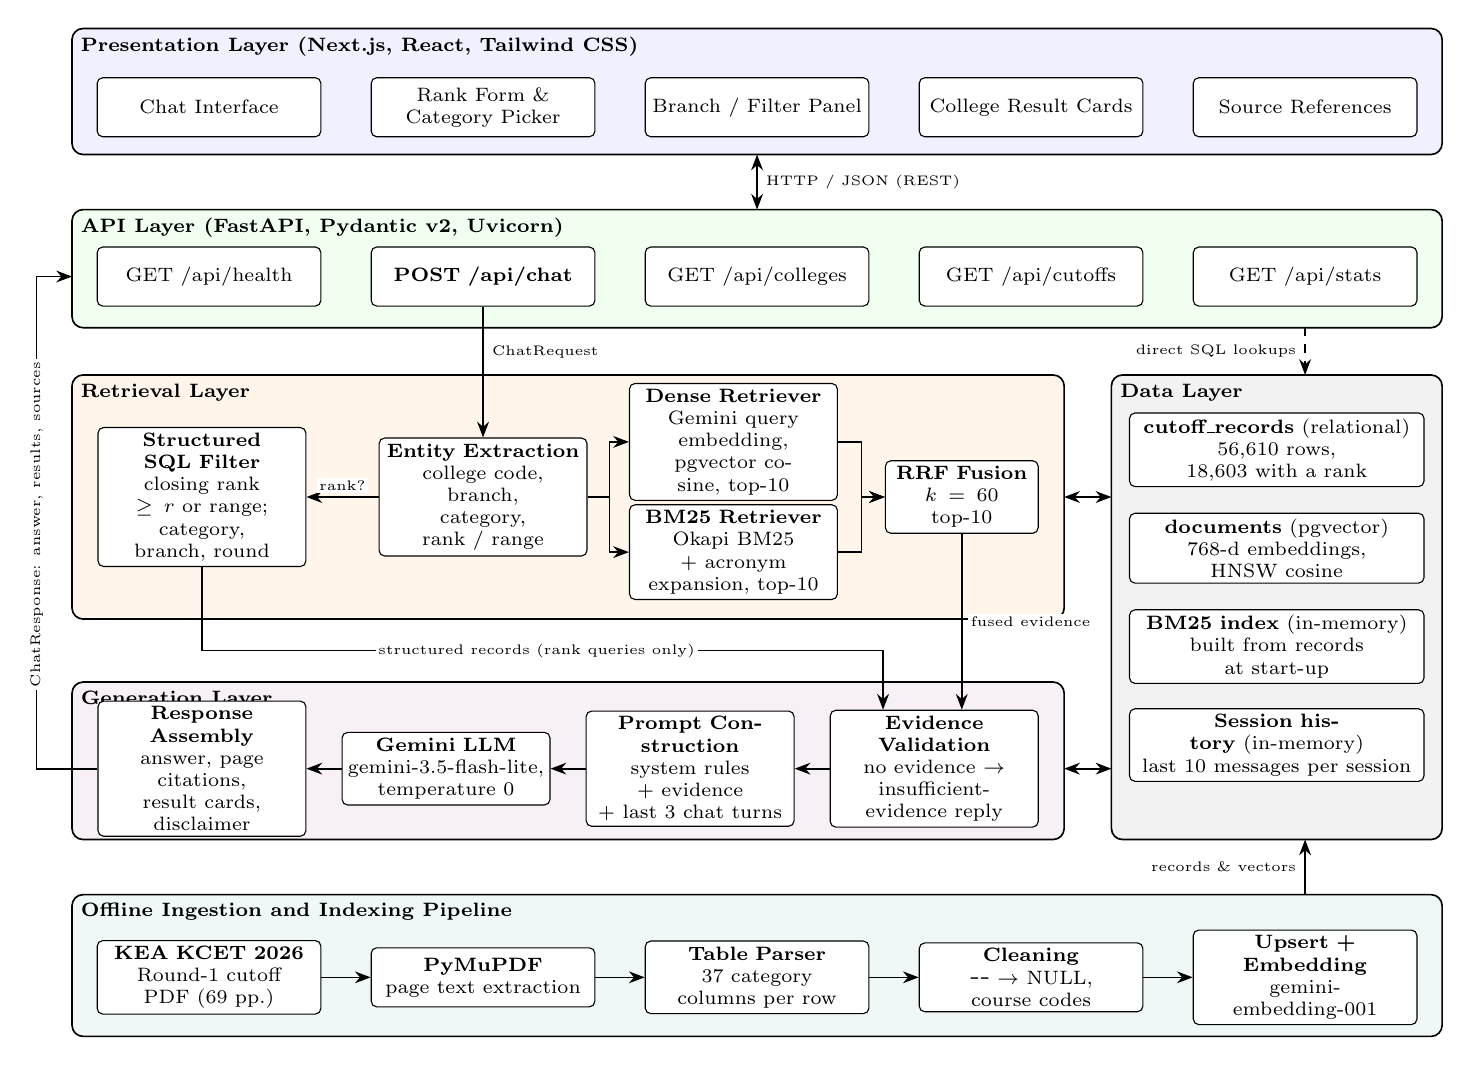
\begin{tikzpicture}[font=\scriptsize]

% ---------- Layer 1: Presentation ----------
\draw[layer, fill=blue!6] (0,0) rectangle (17.4,-1.6);
\node[ltitle] at (0,0) {Presentation Layer (Next.js, React, Tailwind CSS)};
\node[comp] (p1) at (1.74,-1.0)  {Chat Interface};
\node[comp] (p2) at (5.22,-1.0)  {Rank Form \& Category Picker};
\node[comp] (p3) at (8.70,-1.0)  {Branch / Filter Panel};
\node[comp] (p4) at (12.18,-1.0) {College Result Cards};
\node[comp] (p5) at (15.66,-1.0) {Source References};

\draw[darr] (8.70,-1.6) -- (8.70,-2.3)
    node[midway, right=2pt, lbl] {HTTP / JSON (REST)};

% ---------- Layer 2: API ----------
\draw[layer, fill=green!6] (0,-2.3) rectangle (17.4,-3.8);
\node[ltitle] at (0,-2.3) {API Layer (FastAPI, Pydantic v2, Uvicorn)};
\node[comp] (a1) at (1.74,-3.15)  {GET /api/health};
\node[comp] (a2) at (5.22,-3.15)  {\textbf{POST /api/chat}};
\node[comp] (a3) at (8.70,-3.15)  {GET /api/colleges};
\node[comp] (a4) at (12.18,-3.15) {GET /api/cutoffs};
\node[comp] (a5) at (15.66,-3.15) {GET /api/stats};

% ---------- Layer 3: Retrieval ----------
\draw[layer, fill=orange!8] (0,-4.4) rectangle (12.6,-7.5);
\node[ltitle] at (0,-4.4) {Retrieval Layer};
\node[comp=2.5cm] (S) at (1.65,-5.95)
    {\textbf{Structured SQL Filter}\\ closing rank $\geq r$ or range;\\ category, branch, round};
\node[comp=2.5cm] (E) at (5.22,-5.95)
    {\textbf{Entity Extraction}\\ college code, branch,\\ category, rank / range};
\node[comp=2.5cm] (D) at (8.40,-5.25)
    {\textbf{Dense Retriever}\\ Gemini query embedding,\\ pgvector cosine, top-10};
\node[comp=2.5cm] (B) at (8.40,-6.65)
    {\textbf{BM25 Retriever}\\ Okapi BM25 + acronym\\ expansion, top-10};
\node[comp=1.8cm] (R) at (11.30,-5.95)
    {\textbf{RRF Fusion}\\ $k=60$\\ top-10};

\draw[arr] (a2.south) -- (E.north)
    node[pos=0.35, right=2pt, lbl] {ChatRequest};
\draw[arr] (E.west) -- (S.east)
    node[midway, above=1pt, lbl] {rank?};
\draw[arr] (E.east) -- ++(0.28,0) |- (D.west);
\draw[arr] (E.east) -- ++(0.28,0) |- (B.west);
\draw[arr] (D.east) -- ++(0.30,0) |- (R.west);
\draw[arr] (B.east) -- ++(0.30,0) |- (R.west);

% ---------- Layer 4: Generation ----------
\draw[layer, fill=violet!6] (0,-8.3) rectangle (12.6,-10.3);
\node[ltitle] at (0,-8.3) {Generation Layer};
\node[comp=2.5cm] (EV) at (10.95,-9.4)
    {\textbf{Evidence Validation}\\ no evidence $\rightarrow$\\ insufficient-evidence reply};
\node[comp=2.5cm] (PC) at (7.85,-9.4)
    {\textbf{Prompt Construction}\\ system rules + evidence\\ + last 3 chat turns};
\node[comp=2.5cm] (G) at (4.75,-9.4)
    {\textbf{Gemini LLM}\\ gemini-3.5-flash-lite,\\ temperature 0};
\node[comp=2.5cm] (RA) at (1.65,-9.4)
    {\textbf{Response Assembly}\\ answer, page citations,\\ result cards, disclaimer};

\coordinate (sqlx) at (10.30,0);
\draw[arr] (R.south) -- (R.south |- EV.north)
    node[pos=0.5, right=2pt, lbl] {fused evidence};
\draw[arr] (S.south) -- (1.65,-7.9) -- (10.30,-7.9) -- (EV.north -| sqlx);
\node[lbl] at (5.9,-7.9) {structured records (rank queries only)};
\draw[arr] (EV.west) -- (PC.east);
\draw[arr] (PC.west) -- (G.east);
\draw[arr] (G.west) -- (RA.east);

% response path back to the API layer
\draw[arr] (RA.west) -- (-0.45,-9.4) -- (-0.45,-3.15) -- (0,-3.15);
\node[lbl, rotate=90] at (-0.45,-6.3) {ChatResponse: answer, results, sources};

% ---------- Data layer ----------
\draw[layer, fill=gray!10] (13.2,-4.4) rectangle (17.4,-10.3);
\node[ltitle] at (13.2,-4.4) {Data Layer};
\node[comp=3.6cm] (D1) at (15.3,-5.35)
    {\textbf{cutoff\_records} (relational)\\ 56,610 rows, 18,603 with a rank};
\node[comp=3.6cm] (D2) at (15.3,-6.6)
    {\textbf{documents} (pgvector)\\ 768-d embeddings, HNSW cosine};
\node[comp=3.6cm] (D3) at (15.3,-7.85)
    {\textbf{BM25 index} (in-memory)\\ built from records at start-up};
\node[comp=3.6cm] (D4) at (15.3,-9.1)
    {\textbf{Session history} (in-memory)\\ last 10 messages per session};

\draw[darr] (12.6,-5.95) -- (13.2,-5.95);
\draw[darr] (12.6,-9.4) -- (13.2,-9.4);
\draw[arr, dashed] (15.66,-3.8) -- (15.66,-4.4)
    node[midway, left=2pt, lbl] {direct SQL lookups};

% ---------- Offline ingestion ----------
\draw[layer, fill=teal!6] (0,-11.0) rectangle (17.4,-12.8);
\node[ltitle] at (0,-11.0) {Offline Ingestion and Indexing Pipeline};
\node[comp] (I1) at (1.74,-12.05)
    {\textbf{KEA KCET 2026}\\ Round-1 cutoff PDF (69 pp.)};
\node[comp] (I2) at (5.22,-12.05)
    {\textbf{PyMuPDF}\\ page text extraction};
\node[comp] (I3) at (8.70,-12.05)
    {\textbf{Table Parser}\\ 37 category columns per row};
\node[comp] (I4) at (12.18,-12.05)
    {\textbf{Cleaning}\\ \texttt{-{}-} $\rightarrow$ NULL, course codes};
\node[comp] (I5) at (15.66,-12.05)
    {\textbf{Upsert + Embedding}\\ gemini-embedding-001};
\draw[arr] (I1.east) -- (I2.west);
\draw[arr] (I2.east) -- (I3.west);
\draw[arr] (I3.east) -- (I4.west);
\draw[arr] (I4.east) -- (I5.west);
\draw[arr] (15.66,-11.0) -- (15.66,-10.3)
    node[midway, left=2pt, lbl] {records \& vectors};

\end{tikzpicture}%
}
\caption{Layered architecture of the proposed KCET college information
chatbot. Solid arrows show the online request path; the offline pipeline
populates the data layer once per cutoff document.}
\label{fig:architecture}
\end{figure*}

\begin{enumerate}
    \item \textit{Presentation layer:} a Next.js web interface
    providing a chat window, a rank and category form, a branch
    filter, result cards for matching colleges, and a source
    reference panel.

    \item \textit{API layer:} a FastAPI service. The
    \texttt{POST /api/chat} endpoint runs the full RAG pipeline,
    while \texttt{/api/colleges}, \texttt{/api/cutoffs}, and
    \texttt{/api/stats} answer simple browsing requests directly
    from the database.

    \item \textit{Retrieval layer:} entity extraction, the dense
    and BM25 retrievers, RRF fusion, and the structured SQL filter.

    \item \textit{Generation layer:} evidence validation, prompt
    construction, Gemini generation, and response assembly.

    \item \textit{Data layer:} a Neon-hosted PostgreSQL database
    with relational cutoff records and a pgvector document table,
    together with an in-memory BM25 index and a short in-memory
    conversation history.
\end{enumerate}

The offline ingestion pipeline runs once for each cutoff
document and populates the data layer.

% ------------------------------------------------
% 5. METHODOLOGY
% ------------------------------------------------
\section{Methodology}

The methodology consists of an offline indexing phase
(Sections~\ref{sec:ingest}--\ref{sec:index}) and an online
query-processing phase (Sections~\ref{sec:entity}--\ref{sec:gen}).
The online phase is summarised in Fig.~\ref{fig:flow} and
Algorithm~\ref{alg:pipeline}.

\subsection{Data Acquisition and Ingestion}
\label{sec:ingest}

The knowledge source is the official KEA ``UGCET-2026
Provisional Allotment Cut-off Ranks'' document for engineering,
Round~1, General (Rest of Karnataka) seats. Table~\ref{tab:dataset}
summarises the dataset.

\begin{table}[!t]
\centering
\caption{Dataset Summary}
\label{tab:dataset}
\footnotesize
\renewcommand{\arraystretch}{1.1}
\begin{tabular}{@{}lr@{}}
\toprule
\textbf{Attribute} & \textbf{Value} \\
\midrule
Source document pages & 69 \\
Admission year / counselling round & 2026 / Round 1 \\
Seat region & Rest of Karnataka \\
Colleges & 242 \\
College--course combinations & 1,530 \\
Reservation categories & 37 \\
Total college--course--category records & 56,610 \\
Records with a published closing rank & 18,603 (32.9\%) \\
Records without a rank (stored as NULL) & 38,007 \\
\bottomrule
\end{tabular}
\end{table}

Text is extracted page by page using PyMuPDF. Because each
table row is laid out as a course name followed by 37 numeric
rank columns, a token-stream parser is used instead of a
generic table extractor. The parser:

\begin{itemize}
    \item detects college headers (``College: E001 \ldots'')
    and records the current college code, name, and location;
    \item skips repeated page headers and footers;
    \item reads the course name tokens, followed by exactly
    37 rank tokens, one per reservation category;
    \item repairs decimal ranks that are split across lines
    by the PDF renderer; and
    \item logs rows whose rank count differs from 37 for
    manual inspection.
\end{itemize}

During cleaning, missing ranks (\texttt{-{}-}) are stored as NULL and
never as zero, so that they cannot be mistaken for a valid rank.
Course names are mapped to standard branch codes (for example,
\texttt{CS}, \texttt{IS}, \texttt{EC}) using an ordered set of
regular-expression rules, and the college location is identified
from a list of Karnataka cities. Each record retains its page
number for citation. Records are deduplicated on
(college, course, category, year, round, region) and inserted into
the \texttt{cutoff\_records} table using batched upserts.

\subsection{Record-Level Document Construction}

Fixed-size text chunking is not suitable for tabular cutoff data,
because a chunk boundary can separate a rank from its college,
course, or category. Instead, each record with a published
closing rank is converted into one self-contained document:

\begin{center}
\begin{minipage}{0.92\columnwidth}
\footnotesize\ttfamily
College Code: E001\\
College Name: University Visvesvaraya College of Engineering \ldots\\
Location: Bangalore\\
Course Code: AD\\
Course Name: Artificial Intelligence and Data Science\\
Category: 1G \quad Closing Rank: 6475\\
Year: 2026 \quad Counselling Round: 1\\
Seat Region: Rest of Karnataka \quad Page: 1
\end{minipage}
\end{center}

A JSON metadata object containing the same fields is stored
with each document. It is used for metadata filtering and for
generating source citations. This produces 18,603 retrievable
documents.

\subsection{Indexing}
\label{sec:index}

\textit{Dense index:} documents are embedded with the Gemini
\texttt{gemini-embedding-001} model using the
\texttt{retrieval\_document} task type and an output dimension of
768. Embeddings are generated in batches of 50 with exponential
back-off on rate-limit errors, and stored in the \texttt{documents}
table using pgvector. A Hierarchical Navigable Small World (HNSW)
index with cosine distance is created for approximate
nearest-neighbour search.

\textit{Sparse index:} at server start-up, the same document text
is tokenised and loaded into an in-memory \texttt{BM25Okapi} index
from the rank-bm25 library. Tokenisation lower-cases alphanumeric
tokens, preserves short upper-case codes such as \texttt{E005} and
\texttt{2AG}, normalises dotted abbreviations (for example,
``R.\,V.''), and expands common acronyms of colleges (RVCE, MSRIT,
BMSCE, UVCE) and branches (CSE, ISE, ECE, AIML) into their full
terms. The same tokeniser is applied to queries.

\subsection{Query Understanding}
\label{sec:entity}

A rule-based extractor identifies the following entities
in the user's question using regular expressions:

\begin{itemize}
    \item college code (pattern \texttt{E\textbackslash d\{3\}});
    \item reservation category (one of the 37 KEA codes);
    \item a single rank (``rank 5000'') or a rank range
    (``between 5000 and 10000'');
    \item engineering branch, from full names
    (``information science'') or abbreviations (``ISE'').
\end{itemize}

Values selected explicitly in the user interface override the
extracted values. If no category is given, the general merit
category (GM) is used. The resolved category, branch, and
college code form a metadata filter $F$. If an extracted college
code or branch is not already present in the question text, it is
appended to form an enriched query $q'$.

\subsection{Dense Retrieval}

The enriched query is embedded using the
\texttt{retrieval\_query} task type. Documents satisfying the
metadata filter $F$ are ranked by cosine similarity,
\begin{equation}
\mathrm{sim}(q', d) = 1 - d_{\cos}(\mathbf{e}_{q'}, \mathbf{e}_d)
= \frac{\mathbf{e}_{q'} \cdot \mathbf{e}_d}
{\lVert \mathbf{e}_{q'} \rVert \, \lVert \mathbf{e}_d \rVert},
\end{equation}
where $d_{\cos}$ is the pgvector cosine distance. The top 10
documents form the dense ranking $D$.

\subsection{Sparse Retrieval Using BM25}

The BM25 score of a document $d$ for query terms $t \in q'$ is
\begin{equation}
\mathrm{BM25}(q', d) = \sum_{t \in q'} \mathrm{IDF}(t)\,
\frac{f(t,d)\,(k_1 + 1)}
{f(t,d) + k_1\left(1 - b + b\,\frac{|d|}{\mathit{avgdl}}\right)},
\end{equation}
where $f(t,d)$ is the frequency of $t$ in $d$, $|d|$ is the
document length, and $\mathit{avgdl}$ is the average document
length. The library defaults $k_1 = 1.5$ and $b = 0.75$ are used.
Documents with a positive score that satisfy $F$ are sorted, and
the top 10 form the sparse ranking $B$.

\subsection{Hybrid Fusion Using RRF}

The two rankings are fused using Reciprocal Rank Fusion:
\begin{equation}
\mathrm{RRF}(d) = \sum_{r \in \{D, B\}}
\frac{1}{k + \mathrm{rank}_r(d)},
\end{equation}
where $\mathrm{rank}_r(d)$ is the 1-based position of $d$ in
ranking $r$, and a document absent from a ranking contributes
nothing for that ranking. The constant $k = 60$ \cite{Cormack2009}
reduces the score gap between the first few positions, so that a
document ranked moderately well by both retrievers can outrank a
document ranked first by only one. The 10 documents with the highest
fused scores form the hybrid evidence set $H$. Because RRF uses
only rank positions, cosine similarities and BM25 scores do not
need to be normalised to a common scale.

\subsection{Structured Numerical Filtering}

In KCET counselling, a lower rank is better, and a candidate with
rank $r$ could have been allotted a seat only where the closing
rank was at least $r$. When a rank or rank range is detected, the
system therefore queries \texttt{cutoff\_records} directly:
\begin{equation}
Q = \{\, x \mid x.\mathit{cat} = c,\; x.\mathit{branch} = b,\;
x.\mathit{round} = 1,\; x.\mathit{closing} \geq r \,\},
\end{equation}
where records with a NULL closing rank are excluded and the
branch condition is applied only when a branch is specified. For a
range $[r_{\min}, r_{\max}]$, the condition becomes
$r_{\min} \leq x.\mathit{closing} \leq r_{\max}$. The results are
sorted by closing rank in ascending order and limited to 15.
This comparison is performed by the database, not by the
language model.

\subsection{Grounded Response Generation}
\label{sec:gen}

If both $H$ and $Q$ are empty, the system returns a fixed
insufficient-evidence message without calling the language model.
Otherwise, a prompt is constructed from:

\begin{itemize}
    \item a system prompt instructing the model to use only the
    supplied evidence, to state the correct rank-eligibility rule,
    to cite pages, and to end with a disclaimer that past cutoffs
    are not an admission guarantee;
    \item the structured records $Q$ (up to 15);
    \item the fused evidence $H$ (up to 10); and
    \item the last three question--answer turns of the session.
\end{itemize}

The prompt is sent to Gemini (\texttt{gemini-3.5-flash-lite})
with temperature~0. Source references are not taken from the
generated text. Instead, they are built from the page-number
metadata of the evidence records, which guarantees that every
listed reference points to a page of the source document. For
rank queries, the result cards shown to the user are exactly the
SQL matches $Q$; otherwise they are the records in $H$.

\begin{figure}[!t]
\centering
\resizebox{\columnwidth}{!}{%
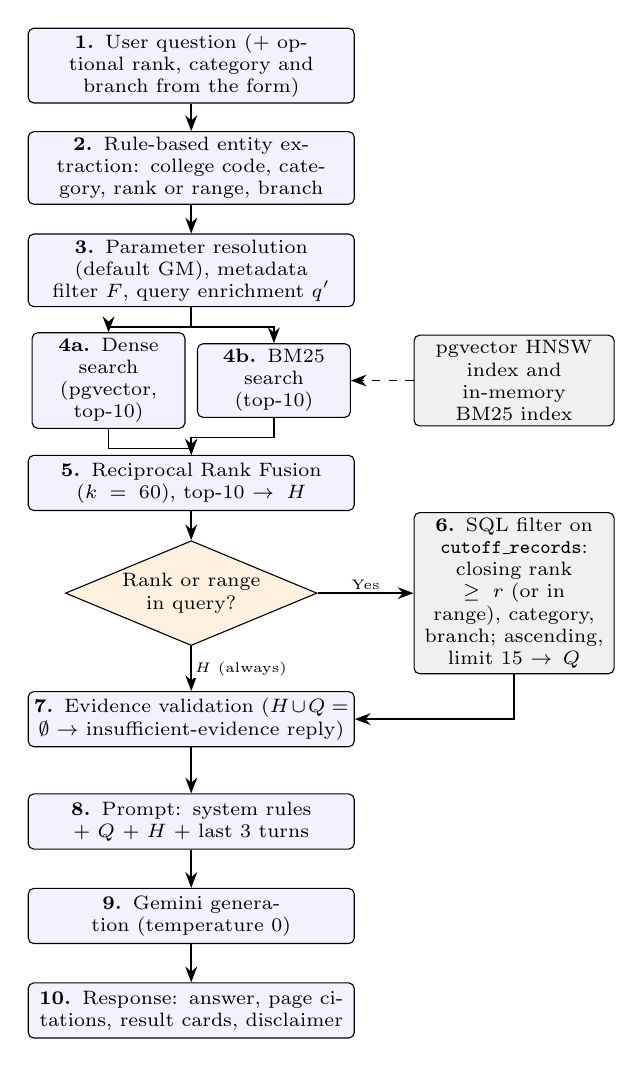
\begin{tikzpicture}[font=\scriptsize]
\node[fcstep] (q) at (-1.2,0)
    {\textbf{1.} User question (+ optional rank, category and branch from the form)};
\node[fcstep] (ee) at (-1.2,-1.3)
    {\textbf{2.} Rule-based entity extraction: college code, category, rank or range, branch};
\node[fcstep] (pr) at (-1.2,-2.6)
    {\textbf{3.} Parameter resolution (default GM), metadata filter $F$, query enrichment $q'$};
\node[fcstep=1.8cm] (dn) at (-2.25,-4.0)
    {\textbf{4a.} Dense search (pgvector, top-10)};
\node[fcstep=1.8cm] (bm) at (-0.15,-4.0)
    {\textbf{4b.} BM25 search (top-10)};
\node[fcstep] (rrf) at (-1.2,-5.3)
    {\textbf{5.} Reciprocal Rank Fusion ($k=60$), top-10 $\rightarrow H$};
\node[fcdec] (dc) at (-1.2,-6.7) {Rank or range\\ in query?};
\node[fcside] (sql) at (2.9,-6.7)
    {\textbf{6.} SQL filter on \texttt{cutoff\_records}: closing rank $\geq r$ (or in range), category, branch; ascending, limit 15 $\rightarrow Q$};
\node[fcside] (idx) at (2.9,-4.0)
    {pgvector HNSW index and in-memory BM25 index};
\node[fcstep] (ev) at (-1.2,-8.3)
    {\textbf{7.} Evidence validation ($H \cup Q = \emptyset \rightarrow$ insufficient-evidence reply)};
\node[fcstep] (pc) at (-1.2,-9.6)
    {\textbf{8.} Prompt: system rules + $Q$ + $H$ + last 3 turns};
\node[fcstep] (gen) at (-1.2,-10.8)
    {\textbf{9.} Gemini generation (temperature 0)};
\node[fcstep] (out) at (-1.2,-12.0)
    {\textbf{10.} Response: answer, page citations, result cards, disclaimer};

\draw[arr] (q) -- (ee);
\draw[arr] (ee) -- (pr);
\draw[arr] (pr.south) -- ++(0,-0.25) -| (dn.north);
\draw[arr] (pr.south) -- ++(0,-0.25) -| (bm.north);
\draw[arr] (dn.south) -- ++(0,-0.25) -| (rrf.north);
\draw[arr] (bm.south) -- ++(0,-0.25) -| (rrf.north);
\draw[arr, dashed] (idx.west) -- (bm.east);
\draw[arr] (rrf) -- (dc);
\draw[arr] (dc.east) -- (sql.west) node[midway, above, lbl] {Yes};
\draw[arr] (dc.south) -- (ev.north) node[midway, right, lbl] {$H$ (always)};
\draw[arr] (sql.south) |- (ev.east);
\draw[arr] (ev) -- (pc);
\draw[arr] (pc) -- (gen);
\draw[arr] (gen) -- (out);
\end{tikzpicture}%
}
\caption{Online query-processing workflow. Hybrid retrieval always
runs; SQL filtering is added when the question contains a rank or
rank range.}
\label{fig:flow}
\end{figure}

\begin{algorithm}[!t]
\caption{Hybrid Query Processing}
\label{alg:pipeline}
\footnotesize
\begin{algorithmic}[1]
\Require question $q$; optional rank $r$, category $c$, branch $b$
\Ensure answer $A$, citations $S$, result list $L$
\State $X \gets \textsc{ExtractEntities}(q)$
\State $r \gets r$ \textbf{or} $X.r$; \ $c \gets c$ \textbf{or} $X.c$ \textbf{or} GM; \ $b \gets b$ \textbf{or} $X.b$
\State $F \gets \{c,\ b,\ X.\mathit{code}\}$; \ $q' \gets \textsc{Enrich}(q, X)$
\State $D \gets \textsc{DenseSearch}(q', F, 10)$
\State $B \gets \textsc{BM25Search}(q', F, 10)$
\State $H \gets \textsc{RRF}(D, B, k{=}60, 10)$
\If{$r$ or a rank range is present}
    \State $Q \gets \textsc{SQLFilter}(r, \mathit{range}, c, b)$
\Else
    \State $Q \gets \emptyset$
\EndIf
\If{$H = \emptyset$ \textbf{and} $Q = \emptyset$}
    \State \Return insufficient-evidence message
\EndIf
\State $A \gets \textsc{Gemini}(\textsc{Prompt}(q, Q, H, \mathit{history}))$
\State $S \gets$ page references from the metadata of $Q \cup H$
\State $L \gets Q$ \textbf{if} a rank was given \textbf{else} metadata of $H$
\State \Return $(A, S, L)$
\end{algorithmic}
\end{algorithm}

% ------------------------------------------------
% 6. IMPLEMENTATION
% ------------------------------------------------
\section{Implementation}

Table~\ref{tab:stack} lists the technologies used. The backend is
written in Python and exposes the pipeline through FastAPI. The
retrievers, fusion, SQL service, and generator are implemented as
separate modules so that each can be tested independently, and the
repository includes unit tests for ingestion, embeddings, BM25,
dense retrieval, RRF, the chatbot service, and the API.

\begin{table}[!t]
\centering
\caption{Implementation Stack}
\label{tab:stack}
\footnotesize
\renewcommand{\arraystretch}{1.1}
\begin{tabularx}{\columnwidth}{@{}L{2.3cm}Y@{}}
\toprule
\textbf{Component} & \textbf{Technology} \\
\midrule
Frontend & Next.js, React, TypeScript, Tailwind CSS \\
Backend API & Python, FastAPI, Pydantic v2, Uvicorn \\
PDF extraction & PyMuPDF with a custom token-stream parser \\
Database & Neon PostgreSQL with pgvector (HNSW, cosine) \\
ORM & SQLAlchemy \\
Embeddings & Gemini \texttt{gemini-embedding-001}, 768-d \\
Sparse retrieval & rank-bm25 (\texttt{BM25Okapi}) \\
Fusion & Custom RRF implementation, $k=60$ \\
LLM & Gemini \texttt{gemini-3.5-flash-lite}, temperature 0, via LangChain \\
Testing & Pytest, HTTPX \\
\bottomrule
\end{tabularx}
\end{table}

% ------------------------------------------------
% 7. EVALUATION METHODOLOGY
% ------------------------------------------------
\section{Evaluation Methodology}

The system is evaluated at both the retrieval and
response-generation levels.

\subsection{Retrieval Evaluation}

A benchmark of 15 in-domain questions was constructed. Each
question names a college (by full name, acronym, or code), a
branch, and optionally a category. A retrieved record is considered
relevant if its college code and branch both match the expected
values. The dense, BM25, and hybrid rankings are produced for the
same query, and the top $K=5$ results of each are scored using:

\textbf{Precision@K:} the proportion of relevant records among the
top $K$ results.
\begin{equation}
\mathrm{Precision@}K =
\frac{\text{relevant records in top } K}{K}
\end{equation}

\textbf{Hit Rate@K:} the fraction of queries for which at least one
relevant record appears in the top $K$ results.
\begin{equation}
\mathrm{Hit@}K = \frac{1}{N}\sum_{i=1}^{N}
\mathbb{1}\left[\,\exists\, j \leq K : d_{ij} \text{ is relevant}\,\right]
\end{equation}

\textbf{Mean Reciprocal Rank (MRR):} the mean reciprocal rank of
the first relevant record.
\begin{equation}
\mathrm{MRR} =
\frac{1}{N}
\sum_{i=1}^{N}
\frac{1}{\mathrm{rank}_i}
\end{equation}
where $\mathrm{rank}_i$ is the position of the first relevant
record for query $i$, and the term is zero if no relevant record
is retrieved.

% Results table: uncomment after re-running scripts/evaluate_retrieval.py
% with verified ground-truth college codes.
%
% \begin{table}[!t]
% \centering
% \caption{Retrieval Results on the 15-Query Benchmark ($K=5$)}
% \label{tab:results}
% \footnotesize
% \begin{tabular}{@{}lccc@{}}
% \toprule
% \textbf{Retriever} & \textbf{P@5} & \textbf{Hit@5} & \textbf{MRR} \\
% \midrule
% Dense (pgvector) & -- & -- & -- \\
% BM25             & -- & -- & -- \\
% Hybrid (RRF)     & -- & -- & -- \\
% \bottomrule
% \end{tabular}
% \end{table}

\subsection{Response Evaluation}

Generated responses are evaluated using the following criteria:

\begin{itemize}
    \item Faithfulness: whether the generated
    answer is supported by the retrieved evidence.

    \item Answer relevance: whether the response
    addresses the user's question.

    \item Context relevance: whether the retrieved
    information is relevant to the query.

    \item Source accuracy: whether the cited
    pages contain the stated closing ranks.

    \item Out-of-domain handling: whether the system declines
    questions outside its scope (for example, medical or JEE
    cutoffs). Five such questions are included in the benchmark.
\end{itemize}

RAGAS \cite{RAGAS2023} and ARES \cite{ARES2024} provide
established approaches for measuring these aspects of
retrieval-augmented generation. For rank-eligibility questions,
the SQL results can also be checked exactly against the source
document, because the eligibility rule is deterministic.

% ------------------------------------------------
% 8. LIMITATIONS
% ------------------------------------------------
\section{Limitations}

\begin{itemize}
    \item The current knowledge base covers a single year, a single
    counselling round, and a single seat region. Trends across years
    cannot yet be analysed.

    \item Entity extraction is rule-based. Questions phrased in
    unexpected ways, or containing spelling errors, may not have
    their rank, category, or branch detected.

    \item When no category is specified, the system assumes GM,
    which may not match the user's actual category.

    \item Out-of-domain questions are handled only through the
    system prompt; there is no separate query classifier.

    \item Conversation history is stored in server memory and is
    lost when the server restarts.

    \item Mapping course names to standard branch codes may merge
    closely related specialisations under one code.
\end{itemize}

% ------------------------------------------------
% 9. CONCLUSION
% ------------------------------------------------
\section{Conclusion}

This paper presents an AI-powered college
information chatbot designed to assist engineering
aspirants in Karnataka by providing access to
official KCET cutoff information.

The official cutoff document is converted into structured
records and record-level documents. The proposed architecture
combines dense semantic retrieval with BM25-based sparse retrieval,
fuses the two rankings using Reciprocal Rank Fusion, and uses
deterministic SQL filtering for rank-eligibility queries. The
retrieved evidence is supplied to Google Gemini to generate
natural-language responses, while source references are derived
from record metadata.

The literature review establishes the relevance
of RAG, hybrid information retrieval, rank fusion,
and educational chatbot systems to the proposed
architecture.

Future work includes adding cutoff documents from multiple years
and counselling rounds, replacing rule-based entity extraction with
a learned or LLM-based parser, adding a cross-encoder reranker,
reporting retrieval results on a larger verified benchmark, and
conducting a user study with KCET aspirants.

% ------------------------------------------------
% REFERENCES
% ------------------------------------------------
\begin{thebibliography}{99}

\bibitem{Lewis2020}
P. Lewis, E. Perez, A. Piktus, F. Petroni,
V. Karpukhin, N. Goyal, H. K\"uttler,
M. Lewis, W.-T. Yih, T. Rockt\"aschel,
S. Riedel, and D. Kiela,
``Retrieval-Augmented Generation for
Knowledge-Intensive NLP Tasks,''
in \emph{Advances in Neural Information
Processing Systems}, vol. 33, 2020,
pp. 9459--9474.

\bibitem{REALM2020}
K. Guu, K. Lee, Z. Tung, P. Pasupat,
and M.-W. Chang,
``Retrieval Augmented Language Model
Pre-Training,''
in \emph{Proceedings of the 37th
International Conference on Machine Learning},
PMLR, vol. 119, 2020, pp. 3929--3938.

\bibitem{Robertson2009}
S. Robertson and H. Zaragoza,
``The Probabilistic Relevance Framework:
BM25 and Beyond,''
\emph{Foundations and Trends in Information
Retrieval}, vol. 3, no. 4, pp. 333--389, 2009,
doi: 10.1561/1500000019.

\bibitem{Cormack2009}
G. V. Cormack, C. L. A. Clarke,
and S. Buettcher,
``Reciprocal Rank Fusion Outperforms
Condorcet and Individual Rank Learning
Methods,''
in \emph{Proceedings of the 32nd ACM SIGIR
Conference on Research and Development
in Information Retrieval}, 2009,
pp. 758--759,
doi: 10.1145/1571941.1572114.

\bibitem{Karpukhin2020}
V. Karpukhin, B. Oguz, S. Min, P. Lewis,
L. Wu, S. Edunov, D. Chen, and W.-T. Yih,
``Dense Passage Retrieval for Open-Domain
Question Answering,''
in \emph{Proceedings of EMNLP}, 2020,
pp. 6769--6781,
doi: 10.18653/v1/2020.emnlp-main.550.

\bibitem{ColBERT2020}
O. Khattab and M. Zaharia,
``ColBERT: Efficient and Effective Passage
Search via Contextualized Late Interaction
over BERT,''
in \emph{Proceedings of the 43rd International
ACM SIGIR Conference on Research and
Development in Information Retrieval},
2020, pp. 39--48,
doi: 10.1145/3397271.3401075.

\bibitem{FiD2021}
G. Izacard and E. Grave,
``Leveraging Passage Retrieval with Generative
Models for Open Domain Question Answering,''
in \emph{Proceedings of the 16th Conference
of the European Chapter of the Association
for Computational Linguistics}, 2021,
pp. 874--880,
doi: 10.18653/v1/2021.eacl-main.74.

\bibitem{BEIR2021}
N. Thakur, N. Reimers, A. R\"uckl\'e,
A. Srivastava, and I. Gurevych,
``BEIR: A Heterogeneous Benchmark for
Zero-shot Evaluation of Information
Retrieval Models,''
in \emph{Proceedings of the Neural Information
Processing Systems Track on Datasets and
Benchmarks}, 2021.

\bibitem{RETRO2022}
S. Borgeaud, A. Mensch, J. Hoffmann,
T. Cai, E. Rutherford, K. Millican,
G. B. van den Driessche, J.-B. Lespiau,
B. Damoc, A. Clark, \emph{et al.},
``Improving Language Models by Retrieving
from Trillions of Tokens,''
in \emph{Proceedings of the 39th International
Conference on Machine Learning},
PMLR, vol. 162, 2022,
pp. 2206--2240.

\bibitem{HyDE2023}
L. Gao, X. Ma, J. Lin, and J. Callan,
``Precise Zero-Shot Dense Retrieval without
Relevance Labels,''
in \emph{Proceedings of the 61st Annual
Meeting of the Association for Computational
Linguistics}, 2023, pp. 1762--1777,
doi: 10.18653/v1/2023.acl-long.99.

\bibitem{FLARE2023}
Z. Jiang, F. F. Xu, L. Gao, Z. Sun,
Q. Liu, J. Dwivedi-Yu, Y. Yang,
J. Callan, and G. Neubig,
``Active Retrieval Augmented Generation,''
in \emph{Proceedings of EMNLP}, 2023,
pp. 7969--7992,
doi: 10.18653/v1/2023.emnlp-main.495.

\bibitem{RAGAS2023}
S. Es, J. James, L. Espinosa-Anke,
and S. Schockaert,
``RAGAS: Automated Evaluation of Retrieval
Augmented Generation,''
in \emph{Proceedings of the 18th Conference of the
European Chapter of the Association for
Computational Linguistics: System Demonstrations},
2024, pp. 150--158.

\bibitem{LostMiddle2024}
N. F. Liu, K. Lin, J. Hewitt, A. Paranjape,
M. Bevilacqua, F. Petroni, and P. Liang,
``Lost in the Middle: How Language Models
Use Long Contexts,''
\emph{Transactions of the Association for
Computational Linguistics}, vol. 12,
pp. 157--173, 2024,
doi: 10.1162/tacl\_a\_00638.

\bibitem{SelfRAG2024}
A. Asai, Z. Wu, Y. Wang, A. Sil,
and H. Hajishirzi,
``Self-RAG: Learning to Retrieve, Generate,
and Critique through Self-Reflection,''
in \emph{Proceedings of the International
Conference on Learning Representations},
2024.

\bibitem{CRAG2024}
S.-Q. Yan, J.-C. Gu, Y. Zhu,
and Z.-H. Ling,
``Corrective Retrieval Augmented Generation,''
arXiv:2401.15884, 2024.

\bibitem{ARES2024}
J. Saad-Falcon, O. Khattab, C. Potts,
and M. Zaharia,
``ARES: An Automated Evaluation Framework
for Retrieval-Augmented Generation Systems,''
in \emph{Proceedings of NAACL-HLT}, 2024,
pp. 338--354,
doi: 10.18653/v1/2024.naacl-long.20.

\bibitem{CRAGBenchmark2024}
X. Yang, K. Sun, H. Xin, Y. Sun,
N. Bhalla, X. Chen, S. Choudhary,
\emph{et al.},
``CRAG: Comprehensive RAG Benchmark,''
in \emph{Advances in Neural Information
Processing Systems}, vol. 37,
Datasets and Benchmarks Track, 2024.

\bibitem{BlendedRAG2024}
K. Sawarkar, A. Mangal, and S. R. Solanki,
``Blended RAG: Improving RAG
(Retriever-Augmented Generation) Accuracy
with Semantic Search and Hybrid Query-Based
Retrievers,''
arXiv:2404.07220, 2024.

\bibitem{EducationSurvey2025}
J. Swacha and M. Gracel,
``Retrieval-Augmented Generation (RAG)
Chatbots for Education: A Survey of
Applications,''
\emph{Applied Sciences}, vol. 15, no. 8,
Art. no. 4234, 2025,
doi: 10.3390/app15084234.

\bibitem{EducationalRAG2025}
Z. Li, Z. Wang, W. Wang, K. Hung,
H. Xie, and F. L. Wang,
``Retrieval-Augmented Generation for
Educational Application: A Systematic Survey,''
\emph{Computers and Education: Artificial
Intelligence}, vol. 8, Art. no. 100417,
2025,
doi: 10.1016/j.caeai.2025.100417.

\bibitem{LearningSupport2025}
G. Lang and T. G\"urpinar,
``AI-Powered Learning Support: A Study of
Retrieval-Augmented Generation (RAG)
Chatbot Effectiveness in an Online Course,''
\emph{Information Systems Education Journal},
vol. 23, no. 2, pp. 4--13, 2025.

\end{thebibliography}

\end{document}
